\documentclass[a4paper, french, 10pt]{article} % Type du document

% compiler avec : pdflatex, bibtex, pdflatex, pdflatex


% +---------------------------------------------------------------+
% | Language
% +---------------------------------------------------------------+
\usepackage[T1]{fontenc}
\usepackage[utf8]{inputenc}
\usepackage[french]{babel}
\usepackage{graphicx}
\usepackage{multirow}
\usepackage{subfiles}
\usepackage{bytefield}
\usepackage{lastpage}

\usepackage[top=2.5cm, bottom=2.5cm, left=2.5cm, right=2.5cm, showframe=false]{geometry}


%% A PERSONNALISER %%%%%%%%%%%%%%%%%%%%%%%
\renewcommand{\author}{Nathan Miéville}
\newcommand{\prof}{Prof. Marizio Tognolini}
\renewcommand{\title}{Leaf Wetness Sensor}
%%%%%%%%%%%%%%%%%%%%%%%%%%%%%%%%%%%%%%%%%%

\usepackage{fancyhdr}
\setlength{\headheight}{27.06pt}
\pagestyle{fancy}
% Header:
\renewcommand{\headrulewidth}{1pt}
\fancyhead[L]{\title} 
\fancyhead[R]{} 
% Footer:
\pagenumbering{arabic}
\fancyfoot{} % clear all footer fields
\renewcommand{\footrulewidth}{1pt}
\fancyfoot[R]{Page \thepage~/~\pageref{LastPage}} 
\fancyfoot[L]{\author }

\begin{document}

\thispagestyle{empty}

\begin{figure}[ht]
	\begin{minipage}[c]{.49\textwidth}
		
\includegraphics[width=.7\linewidth]{figures/logo_mse}
	\end{minipage}%
	\hfill
	\begin{minipage}[c]{.49\textwidth}
		\raggedleft
		
\includegraphics[width=.65\linewidth]{figures/logo_hesso}
	\end{minipage}%
\end{figure}

\begin{raggedright}
\begin{small}
Master of Science HES-SO in Engineering\\
Av. de Provence 6\\
CH-1007 Lausanne\\
\end{small}
\end{raggedright}

\vfill

\begin{raggedleft}
\begin{huge}
\textbf{Master of Science HES-SO in Engineering}\\
Orientation : Electrical Engineering (EIE)\\
\end{huge}

\vfill

{\Huge \title}\\

\vfill

{\large Fait par}\\[10pt]
{\Huge \textbf{\author}}\\[20pt]
\large Sous la direction de\\
\prof\\
Dans l'Institut d'Automatisation Industrielle de la HEIG-VD
\vfill

\large Lausanne, HES-SO Master, 2022\\
\end{raggedleft}


\newpage
\thispagestyle{empty}
\
\newpage
\thispagestyle{empty}
Accepté par la HES-SO Master (Suisse, Lausanne) sur proposition de\\[10pt]
Professeur \prof, conseiller du projet d'approfondissement\\[30pt]
Lausanne, le \today\\[40pt]

\begin{tabular}{lll}
\prof & \hspace{4cm} & Philippe Barrade\\
Conseiller du PA & \hspace{4cm} & Responsable de la filière Electrical Engineering\\
\end{tabular}

\newpage
\thispagestyle{empty}
\section*{Remerciements}
...

\newpage
\thispagestyle{empty}
\tableofcontents

\newpage

\section{Introduction}
smartfarming, JDC, pluie, humidité, maladies

\section{Etat de l'art}

resistif:
plusieur constructeur:
Davis,Spectrum Caipos Lw
grille mesure electrique:
+ pas cher
- ne détecte pas les fine coute -> peinture
faux positif avec l'humidité

Metos: deux électrode et un tissus -> même problème

capacitif:

Meter (ancienement DECAGON) PHYTOS31 
un des seul du marché beaucoup de revendeur

une expérimentation de: Instrumentation, Sensor and Interfaces Group, Universitat Politècnica de Catalunya, BarcelonaTech, Spain 


\graphicspath{ {./figuresAnalysis} }
\section{Analyse fonctionnel}
\subsection{Besoin}
Afin d'être sûre de commencer dans la bonne direction nous devons définir clairement les besoins auquel notre capteur devra répondre. Comme décrit précédemment, le besoin principal est la prévention du développement de maladie. Il existe des modèles empiriques qui se basent sur le temps d'humidité sur la feuille. Cette variable est difficile à déterminer par les données météo classique (humidité, température, vents etc). Le recours à un capteur d'humectation est utile dans ce cas là.
Un autre besoin est pour l'aide aux traitement. La plupart des traitements chimiques d'une plantation doivent être effectués lorsque les feuilles sont sèches. Un capteur d'humectation doit permettre de fournir cette information rapidement.  

\begin{figure}[!ht]
 \centering
 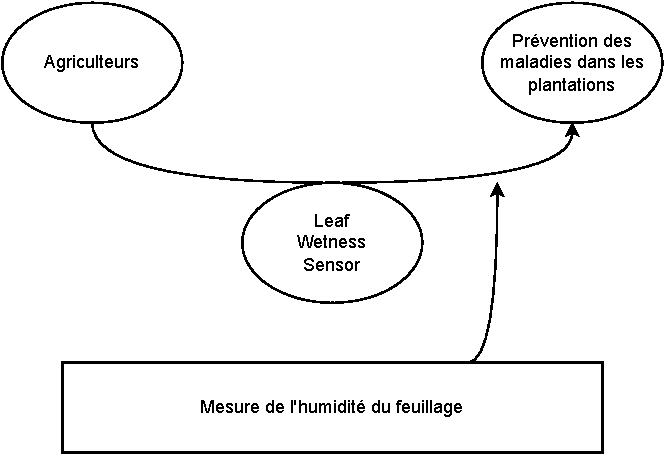
\includegraphics{DiagrammeCorne.drawio.pdf}
 \caption{Le besoin principale exprimé sous la forme d'un diagramme bête à cornes.}
\end{figure}

\subsection{Fonction principale et contrainte }

Pour répondre aux besoins, la fonction principale sera de mesurer l'humectation des feuilles. Cette fonction s'accompagne de plusieurs contraintes apportées par l’environnement dans lequel s'inscrit le capteur. Pour être sûre de n'en oublier aucune, nous nous aidons d'un diagramme pieuvre. 

\begin{description}
 \item[FC1] Il est développé dans le cadre du projet JDC Smart Farming. Il devra être compatible avec le système déjà créé. 
 \item[FC2] Il sera déployé dans des plantations avec une batterie comme source d'énergie. La consommation doit être contrôlée.   
 \item[FC3] En extérieur la météo peut faire varier l’environnement du capteur. Il devra être robuste à ces changements pour qu'il n’influence pas les mesures.
 \item[FC4] Les intempéries que subira le capteur ne doivent pas l’endommager ou compromettre les mesures.
 \item[FC5] Dans les plantations, il y a régulièrement des tracteurs et des machines qui passent entre les plantes. Le capteur ne doit pas gêner ou être gêner par ces passages. Sa taille doit être contrôlée.
 \item[FC6] L'installation et la maintenance pourra être faite par des agriculteur sans formation technique. Le capteur doit être simple d'installation et de maintenance.
 \item[FC7] Le capteur est développé pour être commercialisé. Il doit répondre aux norme et être certifié.
\end{description}

\newpage

\begin{figure}[!ht]
 \centering
 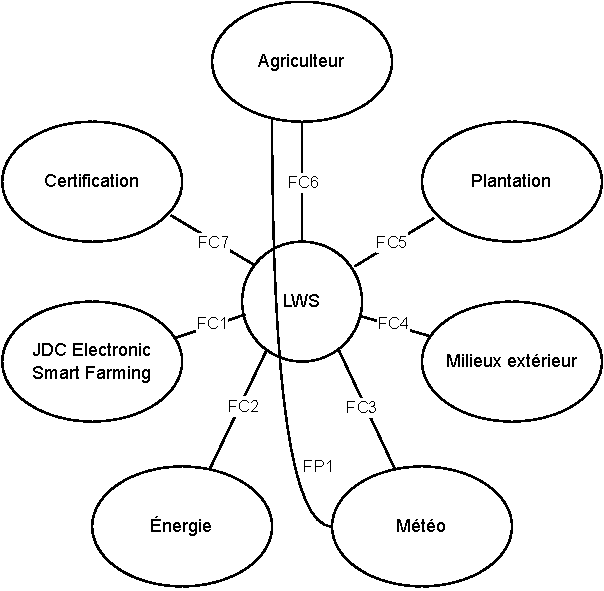
\includegraphics{DiagrammePieuvre.drawio.pdf}
 \caption{Fonctions principales et contraintes sous la forme d'un diagramme pieuvre}
\end{figure}

Après avoir énoncé la fonction principale et toutes les contraintes nous pouvons définir des critères pour chacune d'elles ainsi que des nivaux qui répondent à ces critères. Cela nous permet de construire le cahier des charges auquel nous nous référons pour la conception. 

\paragraph{FP1}
La mesure d'humectation des feuilles se fera au travers d'une mesure de l'humidité relative d'une surface. Elle se donne en pourcentage tel que 0\% correspond à un feuille totalement sèche et 100\% la feuille est entièrement recouverte d'eau. Puisque nous ne connaissons pas encore les performances de notre capteur nous utiliserons la résolution maximale qu'autorise la structure de registre de JDC pour ce type de capteur. La valeur sera stockée sur 1 octet non signé avec une résolution de 0.5\%. La précision est calqué sur la résolution et donne une valeur de 0.25\%. Ces valeur sont très optimistes et nous nous resservons le droit de les changer après une évaluation des performance du capteur plus tard dans le développement. 

\paragraph{FC1} \label{fc1}
L’environnement Smart Farming JDC se compose d'un émetteur LoRa auquels sont reliés plusieurs capteurs au travers d'un bus I2C. Pour que notre capteur soit compatible, il doit impérativement répondre à plusieurs critères. L'interface de sortie doit être évidement un I2C. La structure des registres accessibles est normalisé pour que l’émetteur puisse lire correctement les valeurs afin de les transmettre. Un temps maximal de mesure est défini. Il représente le temps entre le démarrage du capteur jusqu'à que les valeurs de la mesure soit prête. Le capteur devra être câblé sur le connecteur commun à tous les capteurs JDC. Pour finir, l'alimentation fourni par l'émetteur est de 3.3V le capteur devra fonctionner à cette tension.

\paragraph{FC2}
La source d'alimentation du capteur sera une batterie situé aux niveau de l'émetteur. Tous les capteurs d'un même émetteur partage donc la même source. Les capteurs ne sont pas alimentés entre deux mesures. Nous n'avons pas besoin de nous préoccuper de la consommations au repos. En marche, le courant, que nous prendrons comme critère, ne doit pas dépasser 1mA. Ce chiffre avait été calculé par rapport au nombre maximal de capteur ,la capacité de la batterie et l'autonomie souhaité.  

\paragraph{FC3}
Le facteur métrologique qui pourra le plus fausser nos mesures est l'humidité de l'air. Si l'air est chargée en eau, sa constante diélectrique changera et pourra impliquer un augmentation de la capacité alors que la surface est complètement sèche. Pour que ce phénomène n’influence en aucun cas nos mesures, le delta de capacité doit être inférieur à la précision. Cette variation devra être contrôlé et mesurée car elle pourrait dégrader la précision du capteur.   

\paragraph{FC4}
L'utilisation extérieur du capteur nécessite qu'il soit étanche aux intempéries. Avec la norme IP65 comme objectif, le capteur sera suffisamment protéger des plus grosses pluies ainsi que des traitements pulvérisés sur les cultures.    

\paragraph{FC5}
Pour s’intégrer aux mieux dans les plantations le capteur ne devra pas être trop volumineux. Nous prendrons arbitrairement une envergure maximum de 20 cm. Cela correspond à une moyenne des capteur existant sur le marché.

\paragraph{FC6}
La facilité d'installation a déjà été pensée et est garantie par la contrainte \textbf{FC1}.

\paragraph{FC7}
Pour être proposé sur le marché le capteur doit être certifié. Il doit possédé le CE pour être distribué en Europe et une certification de compatibilité électromagnétique pour garantir que le capteur respecte les normes en vigueur.  

\bigskip
Le cahier des charge résume tous les critères et leur niveau pour chaque contrainte.

\begin{table}[!h]
\begin{center}
\resizebox{\columnwidth}{!}{%
\begin{tabular}{|l|l|p{5cm}|l|}
\hline
 & \textbf{Fonctions} & \textbf{Critères} & \textbf{Niveaux}\\
\hline
\textbf{FP1} &Mesurer l'humectation des feuilles & Mesure d'humidité relative d'une surface & RH de 0\% à 100\%  résolution de 0.5\%  précision +- 0.25\%\\
\hline
\multirow{5}{*}{\textbf{FC1}} & S'intégrer dans l'environnement Smart Farming JDC & Interface  de sortie I2C & Baud rate 100KHz. Adresse configurable\\\cline{3-4}
 &  & Structure de registre normalisé, & (voir doc JDC)\\\cline{3-4}
 &  & Démarrage de la mesure et acquisition après un temps. & 50ms pour la capture de la mesure\\\cline{3-4}
 &  & Connecteur JDC & Sortie 4 fil avec  VCC,GND,SDA,SCL\\\cline{3-4}
 &  & Alimentation normalisé & Tesion 3.3V\\\cline{3-4}
\hline
\textbf{FC2} & Consommer peu d'énergie & Courant maximum établit en fonctionnement & 1 mA\\
\hline
\textbf{FC3} & Eviter les faux positifs du à la météorologie & L'humidité de l'air ne doit pas influencer la mesure & L'incidence de RH de l'air < précision (0.25\%)\\
\hline
\textbf{FC4} & Résister aux milieux extérieurs & Le capteur est protégé des intempéries et supporte une utilisation extérieur & Etanche IP65\\
\hline
\textbf{FC5} & S'intègrer dans les plantations & La taille du capteur ne doit pas gêner l'exploitation des plantations & Envergure maximum de 20cm\\
\hline
\textbf{FC6} & Etre facile d'installation & Le capteur doit pouvoir être installer par des agriculteurs sans formation technique & Système d'attache et un seul connecteur à brancher\\
\hline
\textbf{FC7} & Etre Certifié & Le capteur doit être certifié pour être proposé sur le marché & Certification EMC,CE\\
\hline
\end{tabular}
}
\end{center}
\caption{Cahier des charges}
\end{table}

\newpage

\subsection{Architecture du système}

En nous basant sur le cahier des charges, nous pouvons commencer à concevoir l'architecture de notre capteur. Pour nous aider dans cette tâche nous utiliserons un diagramme FAST. Il nous permettra méthodiquement de faire la liste de tous les éléments nécessaires au bon fonctionnement du capteur.

\begin{figure}[!ht]
 \centering
 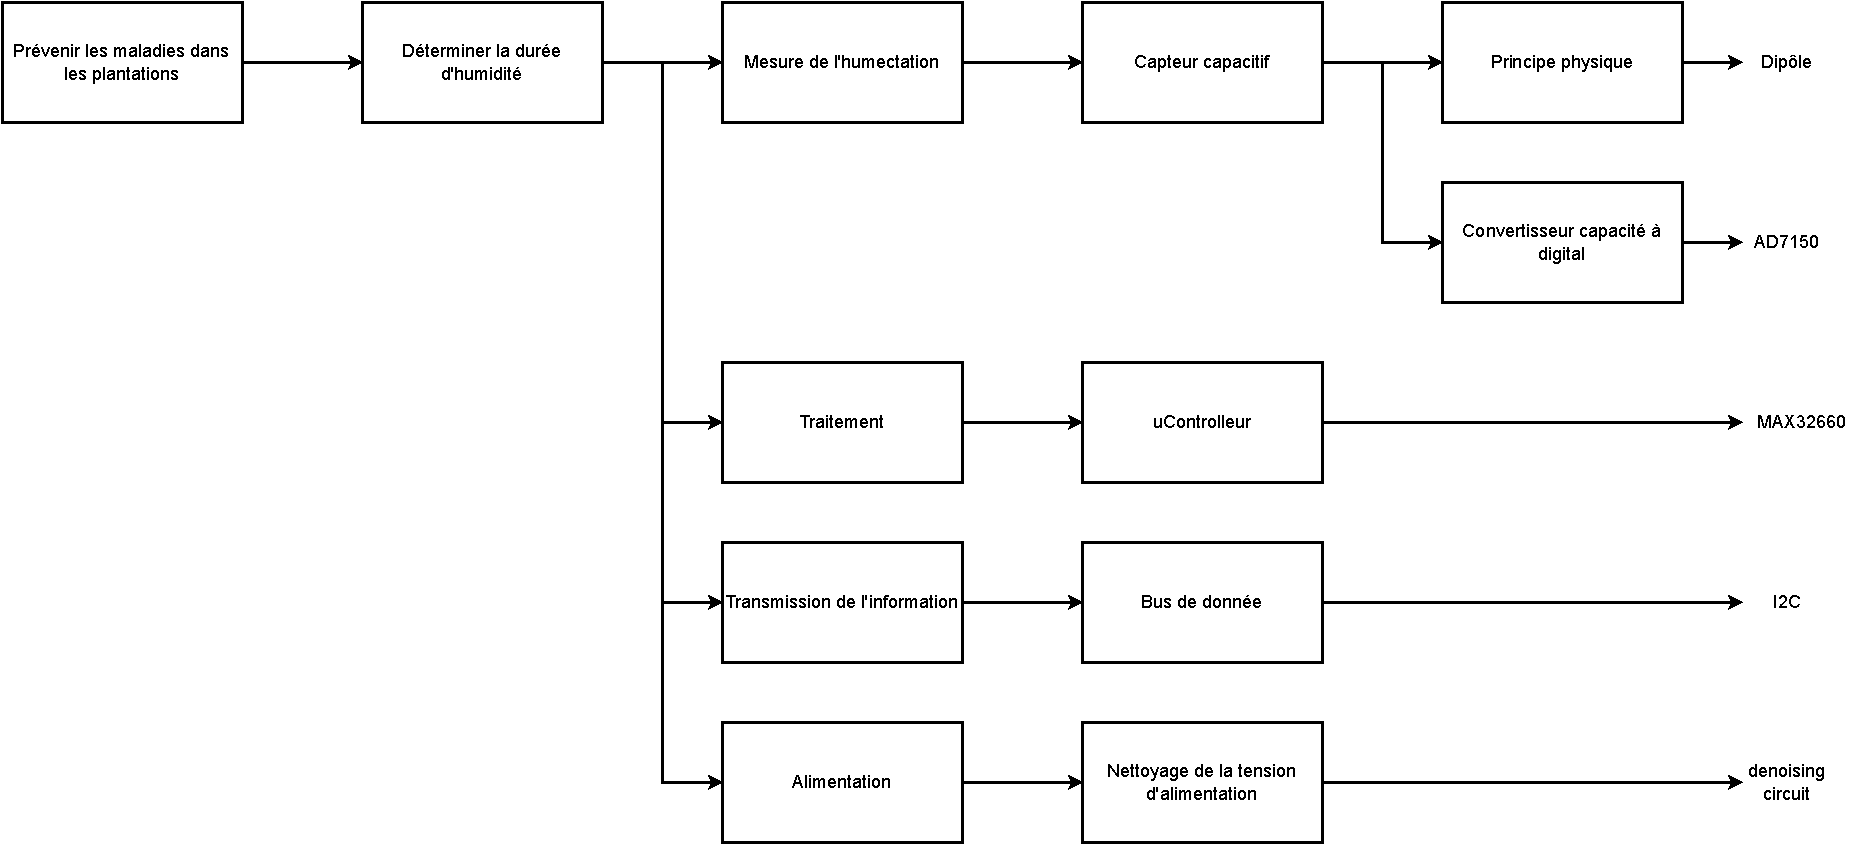
\includegraphics[width=16cm]{DiagrammeFAST.pdf}
 \caption{Diagramme FAST}
\end{figure}

Plusieurs choix techniques ont été fait pendant cette phase d'architecture. Le MAX32660 a été choisi comme micro-contrôleur. JDC l'utilise déjà dans ses capteurs. Plusieurs librairies ont déjà été créés pour intégrer le capteur dans l’environnement JDC ce qui facilitera le développement. Le micro-contrôleur a tous les périphériques que nous avons besoin et est prévu pour la faible consommation. Il ira très bien dans notre application.


l'AD7150 a été choisi parmi les différents convertisseurs capacitifs présentés pendant l'état de l'art. La sélection c'est fait sur la consommation des circuits intégrés. l'AD7745 et le FDC1004 ont une consommation en travail de  \SI{900}{\micro\ampere}. C'est beaucoup trop si on prends en compte le fait qu'un micro-contrôleur s'ajoute à la consommation. Nous serions au-dessus des \SI{1}{\milli\ampere}. l'AD7150 consomme \SI{100}{\micro\ampere} ce qui nous laisse plus de marge. Une carte de développement est disponible à l'achat pour réalisé nos premières mesures. A ce stade il est trop difficile d'estimer la capacité que nous auront à mesurer. Nous prendrons les bornes de ce capteur comme référence pour la création du dipôle. Si nous observons que nous sommes complètement en dehors, nous réévaluerons le choix du convertisseur.

L'alimentation provient du transmetteur et elle est transporté à travers un câble. Pour une mesure correcte, l'alimentation doit être le plus propre possible. Un nettoyage de la tension d'alimentation devra être fait. Nous n'aurons pas l’occasion d'étudier ce circuit dans ce travail car nous utiliserons pour les mesures des cartes de développement qui embarquent leur propre alimentation. Néanmoins, cette partie ne doit pas être négligé pendant la suite du développement.

\newpage
Nous pouvons dès à présent mettre tous nos choix bout à bout pour établir un Schéma block sur lequel nous nous baserons pour la conception. Une recherche dans la datasheet du circuit de mesure de la capacité nous apprend les bornes exacte ainsi que la résolution numérique de la valeur mesurée. Nous pouvons alors tracer la chaîne complète de mesure de notre capteur.

\begin{figure}[!ht]
 \centering
 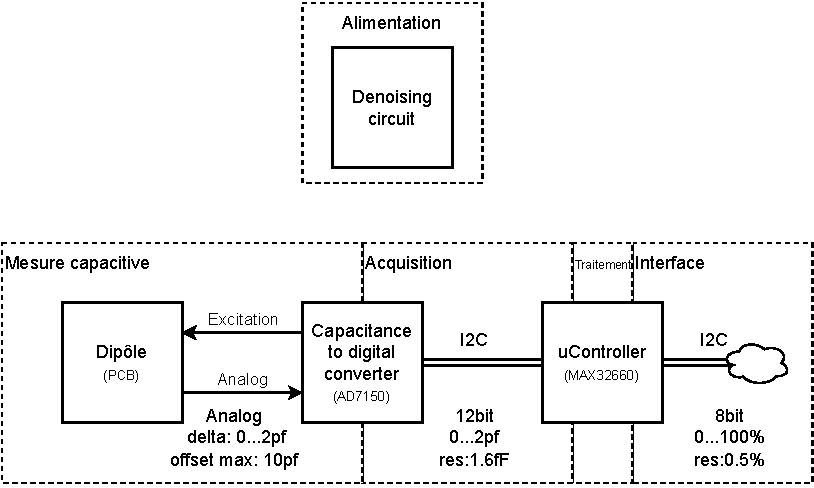
\includegraphics[width=16cm]{SchemaBlock.pdf}
 \caption{Schéma Block}
\end{figure}


\graphicspath{ {./figuresConception} }
\section{Conception}

\subsection{Circuit}
L'objectif de ce travail est d'analyser et de valider le principe physique de notre capteur. Nous nous contrerons principalement sur le dipôle. Nous établissons un schéma électrique du capteur pour nous aider lors du câblage des cartes de développement. Ce schéma ne comporte pas la gestion de l'alimentation car ce qui nous intéresse est la chaîne de mesure.

\begin{figure}[!ht]
 \centering
 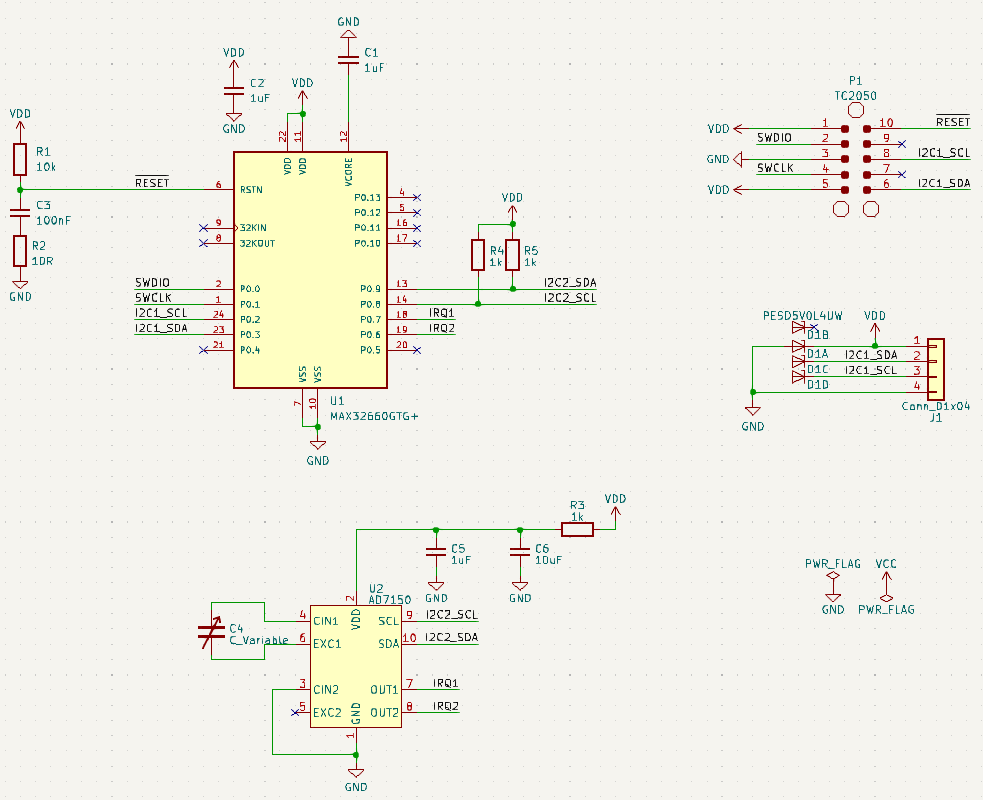
\includegraphics[width=14cm]{schemaelec.png}
 \caption{Schéma électrique}
\end{figure}

Sur ce schéma C4 représente le dipôle. Il est connecter sur le premier port du convertisseur. Un pôle est connecter sur la pin d'excitation et l'autre sur l'entrée analogique. La conversion est faites en excitant d'un côté et en mesurant la charge de l'autre. La valeur est stocké dans un registre prête à être lu par l'I2C. Un filtre conseillé par la datasheet est câblé sur l'alimentation de l'AD7150. Le micro-contrôleur est connecter aux convertisseur par les deux pin de l'I2C, clock et donnée. On utilise le deuxième I2C pour le convertisseur et le premier pour l'interface extérieur. Les pull-up obligatoire sont connecter sur le deuxième I2C mais pas sur le premier car elle se trouve déjà aux niveau de l'émetteur. Les deux sortie numérique sont aussi connecter au micro-contrôleur. Nous ne les utiliserons pas tout de suite mais nous nous en laissons la possibilité. Le connecteur P1 est un tag pour flasher le micro. Il est relié aux pin nécessaire pour sa tâche et à l'I2C d'interface à des fin de debug. Et finalement le connecteur J1 permet de sortir l'interface I2C et apporte l'alimentation. Des diode protège le circuit contre les surtensions.  

\newpage
\subsection{Dipôle}
Le dipôle est la partie de notre capteur qui transforme une variable physique en un paramètre électrique. Dans notre cas il transforme une quantité d'eau sur la surface en une variation de capacité. Pour comprendre comment cela fonctionne il faut comprendre ce qu'est une capacité électrique. $C=\frac{Q}{U}$ défini la capacité (C) comme la charge (Q) stocké par rapport à une tension (U) donné. La capacité d'un dipôle est influencé par trois paramètres. La surface du conducteur l'augmente. La distance entre deux pôle la diminue. Et enfin, Une plus grande permittivité relative du milieux augmentera le milieux. L'eau fera varier ce dernier paramètres ce qui nous laisse les deux autres à définir.

Le dipôle sera d'abord simulé puis mesuré. La simulation se fera avec le logiciel Flux d'Altair. Pour simplifié la simulation nous l’exécuterons en 2 dimension. Ce premier dipôle devra être conçu pour qu'une coupe 2d puisse être utilisé dans la simulation. Nous choisiront un peigne droit en longueur. 

\begin{figure}[!ht]
 \centering
 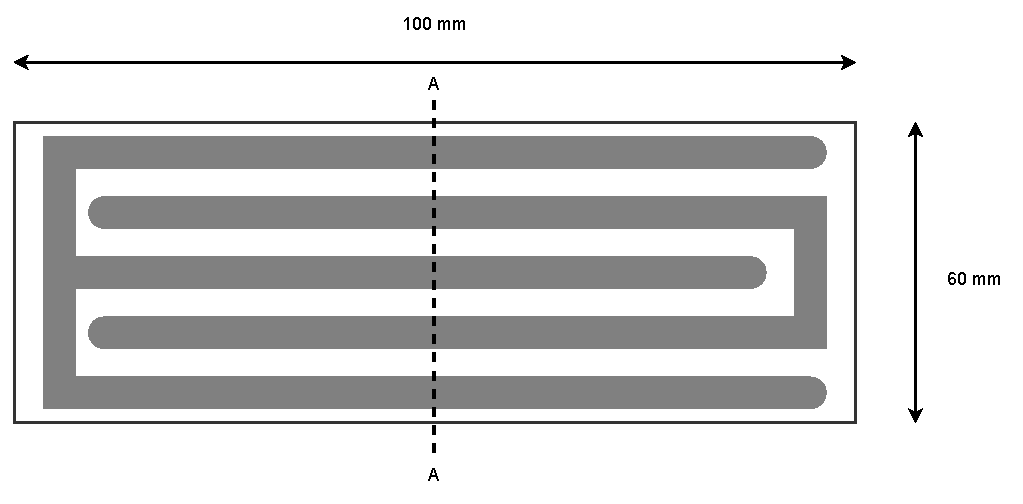
\includegraphics[width=14cm]{dipole-top.pdf}
 \caption{Plan mécanique du dipôle}
 \label{plan}
\end{figure}

Nous avons défini arbitrairement une longueur de 100mm et une largeur de 60mm. Cette taille nous donne un bon compromis entre l'espace disponible sur la carte et le prix de production. 

\begin{figure}[!ht]
 \centering
 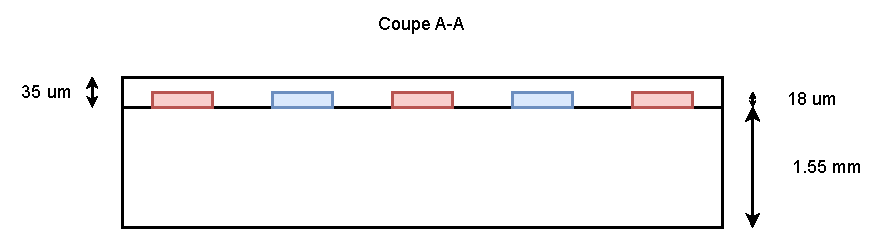
\includegraphics[width=14cm]{dipole-A-A.pdf}
 \caption{Plan mécanique de coupe du dipôle}
 \label{plancoupe}
\end{figure}

Les différentes épaisseurs des couches, du PCB, du cuivre et du masque sont récupéré à partir des dimension de carte standard. C'est cette coupe que nous simulerons dans le logiciel. Cependant nous ajouterons une couche de résine supplémentaire de 0.5 mm d'épaisseur. Elle permettra sur le capteur final de protéger le circuit et d'offrir à l'eau une surface proche de celle de l'eau en terme d'étanchéité et de rugosité. Cette couche ne sera pas présente pour nos première mesures. Mais doit être pris en compte pendant la simulation. Nous évaluerons aussi l'utilisation d'un plan conducteur pour concentré le champs en direction de la surface mesuré et éviter que le capteur sois influencé par ce qui se passe en dessous. Nous prendrons la décision de garder ou non cette couche après l'avoir simulé et étudié.

Le nombre, l'épaisseur, et l'écart des pistes sont des valeurs que nous laissons libre pour la simulation. La coupe ne représente que la partie centrale du PCB. Pour un question de simplicité nous négligerons les extrémité pour les simulations.



\graphicspath{ {./figuresSimulation} }
\section{Simulation}
\subsection{Création du modèle}
Pour simuler notre dipôle nous utiliserons Flux2D d'Altair. La simulation se fait par element fini. Cela consiste à dessiner notre géométrie pour la diviser en plusieurs points grâce à un maillage. Le logiciel résous en chaque point une équation différentiel dérivé des équations de Maxwell pour une application donné. Pour mesurer une capacité nous simulerons dans le domaine de l'électrostatique. Nous nous intéresserons aux charge et aux champs électrique.

\subsubsection{Géométrie}
Flux nous permet de faire du dessin paramétrique. Nous pourrons ainsi, pendant la simulation, faire varier nos paramètre géométrique. Nous créons des paramètres pour toutes nos grandeurs: épaisseur et largeur. La profondeur est entré à la création du modèle. Le logiciel intègre le fait que nous dessinons une coupe et utilisera la profondeur  pour les calcul qui concerne l'ensemble du système comme par exemple l'énergie total. Nous utilisons les valeurs défini pendant la conception, figure \ref{plan} et \ref{plancoupe}. Dans l’intérêt de la simulation nous ajoutons une couche d'eau. Nous ne pouvons pas simulé une goutte en deux dimensions. Nous étudierons un cas sans eau notre 0\% et un cas avec une couche continue notre 100\%. 

Le nombre de piste ne peut pas être paramétrisé car il créer des surfaces supplémentaire, ce qui n'est pas géré en simulation par Flux2D. Nous créerons trois projet pour trois nombre de piste: 20,10,5. Puisque la largeur du circuit et le nombre de pistes est fixe la somme distance et largeur de piste sera fixe aussi. Elle vaudra $S_{piste} = \frac{L_{pcb}}{N_{piste}}$. Si nous changeons la largeur des pistes nous devrons changer la distance. Nous utilisons alors un seul paramètre qui fera varié les deux. Il représente le rapport entre largeur et distance $F_{dist,larg} = \frac{L_{piste}}{D_{piste}} $. Nous pouvons définir largeur et distance en fonction de nos deux nouveau paramètre: $D_{piste} = \frac{S_{piste}}{F_{dist,larg}+1}$, $L_{piste} = S_{piste} - \frac{S_{piste}}{F_{dist,larg}+1}$. C'est ces deux expressions que nous insérons dans le logiciel. 
Une fois tous les paramètre rentré nous construisons avec ceux-ci toute notre géométrie. On crée d'abord les points. Puis on les relie pour former les lignes.  

\begin{table}[!ht]
\begin{center}
\begin{tabular}{|l|l|}
\hline
Paramètre & valeur [mm]\\
\hline
EP\_CIBLE & 2.7\\
\hline
EP\_CUIVRE & 0.018\\
\hline
EP\_MASQUE & 0.035\\
\hline
EP\_PCB & 1.55\\
\hline
EP\_RESINE & 0.5\\
\hline
LARG\_PCB & 60\\
\hline
NBR\_PISTE & 20,10.5\\
\hline
FACTOR\_DIST\_LARG\_PISTE & variable\\
\hline
SUM\_DIST\_LARG\_PISTE & LARG\_PCB/NBR\_PISTE\\
\hline
LARG\_PISTE & {\tiny SUM\_DIST\_LARG\_PISTE-(SUM\_DIST\_LARG\_PISTE/(FACTOR\_DIST\_LARG\_PISTE+1))}\\
\hline
DIST\_PISTE & {\tiny SUM\_DIST\_LARG\_PISTE/(FACTOR\_DIST\_LARG\_PISTE+1)}\\
\hline
\end{tabular}
\caption{Liste des paramètre}
\end{center}
\end{table}

\begin{figure}[!ht]
 \centering
 \includegraphics[width=14cm]{c20geotout.png}
 \caption{Géométrie du modèle entier}
\end{figure}

\begin{figure}[!ht]
 \centering
 \includegraphics[width=14cm]{c20geozoom.png}
 \caption{Géométrie du modèle, zoom sur les pistes}
\end{figure}

\begin{description}
 \item[Bleu Foncé:] couche cible (eau)
 \item[Noir:] Résine
 \item[Vert:] Masque de soudure
 \item[Rouge:] Piste pôle 1
 \item[Bleu claire:] Piste pôle 2
 \item[Brun:] PCB
 \item[Turquoise:] Plan cuivre
\end{description}

Une dernière surface devra être créer pour représenter l'infini. Flux2d fonctionne en appliquant des conditions aux limite sur une sphère défini par l'utilisateur entourant notre modèle. Ces condition permette de simuler un environnement infini dans un zone fini. 

\subsubsection{Physique}
Une fois la géométrie terminé nous pouvons ajouter des contraintes physiques à notre modèle. Cela consiste à assigner des matériaux à nos surfaces. la résine, le masque et le pcb sont des isolant avec une certaine constante diélectrique. Le cuivre sera considéré comme un conducteur parfait. Une tension sera appliqué sur les deux pôle. Nous fixerons un tension de 3.3V et une autre de 1.65V. Cela nous donnera une différence de 1.65V. Nous l’enregistrerons dans un paramètre physique qui pourra être utilisé plus tard dans les calculs. le plan de cuivre restera flottant. l'eau sera aussi considéré comme un isolant avec une constante diélectrique. La cible le plan et la résine pourra être remplacé par de l'aire au besoin de la simulation.


\begin{table}[!ht]
 \begin{center}
\begin{tabular}{|l|l|l|l|}
\hline
Surface & Matériau & $\mu_r$ & Potentiel\\
\hline
Cible & eau & 80 & -\\
\hline
Résine & résine & 4 & -\\
\hline
Masque & résine & 4 & -\\
\hline
Piste P1 & conducteur parfait & - & 3.3 V\\
\hline
Piste P2 & conducteur parfait & - & 1.65 V\\
\hline
PCB & FR4 & 4.4 & -\\
\hline
Plan & conducteur parfait & - & flotant\\
\hline
\end{tabular}
\caption{Caractéristiques physique}
\end{center}
\end{table}



\subsubsection{Maillage}
Le maillage est une partie importante de la création d'un modèle du simulation par élément fini. Un compromis doit être trouvé entre le temps de calcul et la résolution de la simulation. Quelque règle assez simple permettent d'obtenir des résultats convenable. Plus le champs est intense à un endroit plus le maillage doit être fin. Il faut aussi être fin aux intersection entre deux matière. Les grande surface peuvent être plus relâchée aux centre. En suivant ces recommandation j'obtiens un maillage satisfaisant.


\begin{figure}[!ht]
 \centering
 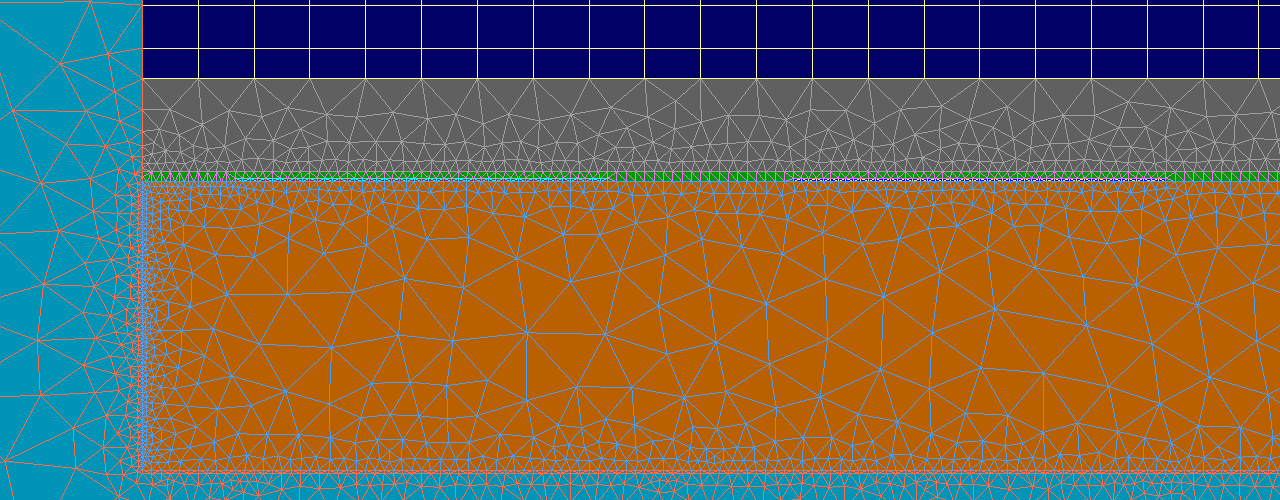
\includegraphics[width=14cm]{C20maillage.png}
 \caption{Maillage du modèle}
\end{figure}


\subsection{Exploitation}

\subsubsection{20 pistes}
Nous pouvons à présent démarrer les simulations. Nous commencerons avec 20 piste et un rapport entre largeur et distance de 2 (largeur des pistes = 2mm, distance entre piste = 1mm). La cible sera de l'air ainsi que le plan. Une fois la simulation terminé nous pouvons afficher le champs magnétique ainsi que les lignes du potentiel électrique pour analysé le résultat et vérifié que la simulation c'est bien passé.

\begin{figure}[!ht]
 \centering
 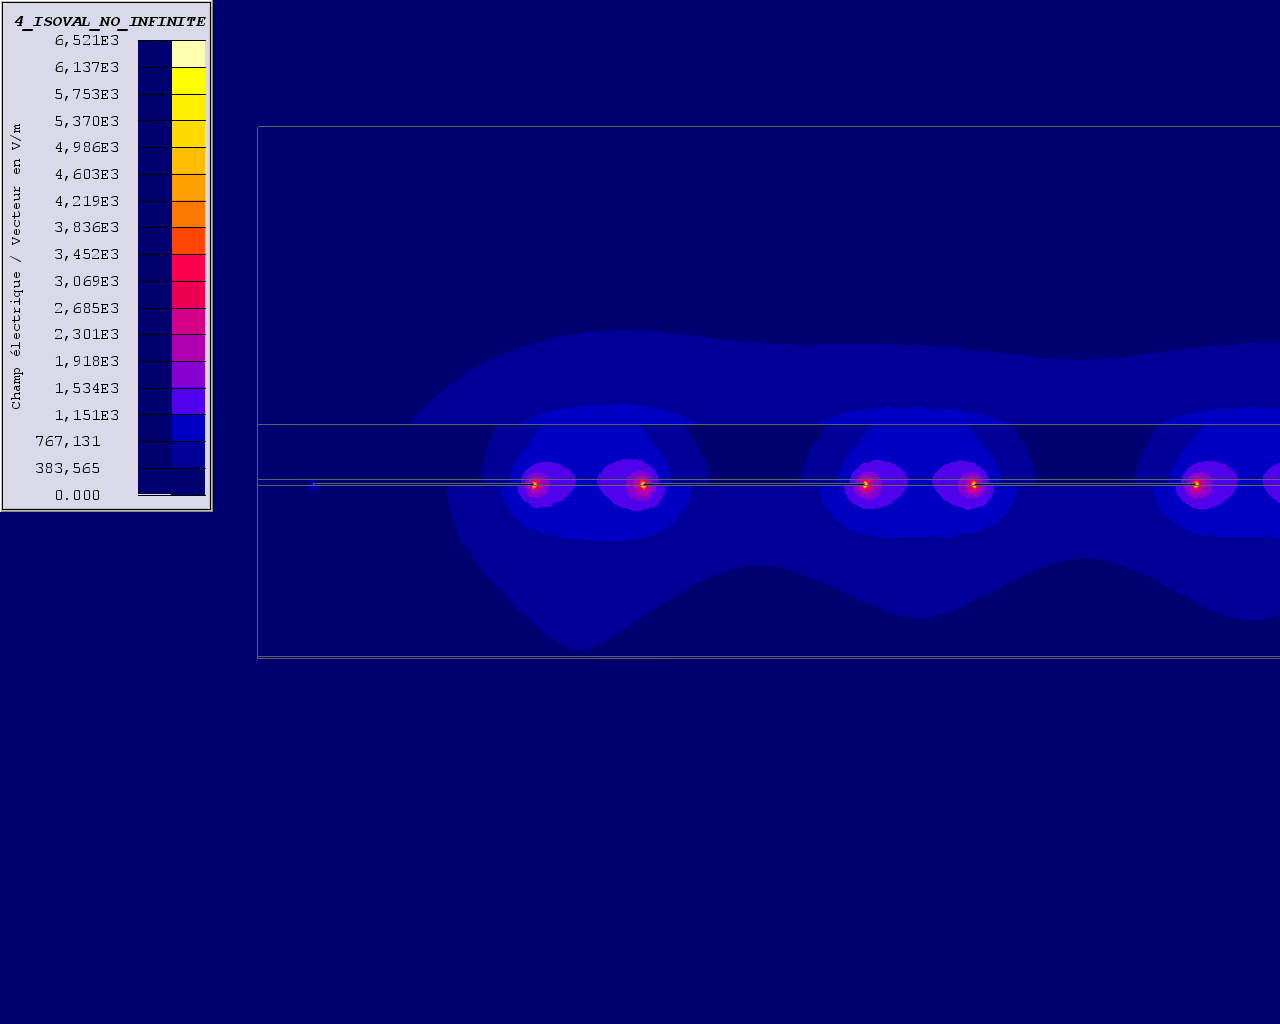
\includegraphics[width=14cm]{simulationChampElectrique.png}
 \caption{Champs électrique 20 pistes}
\end{figure}

\newpage
\begin{figure}[!ht]
 \centering
 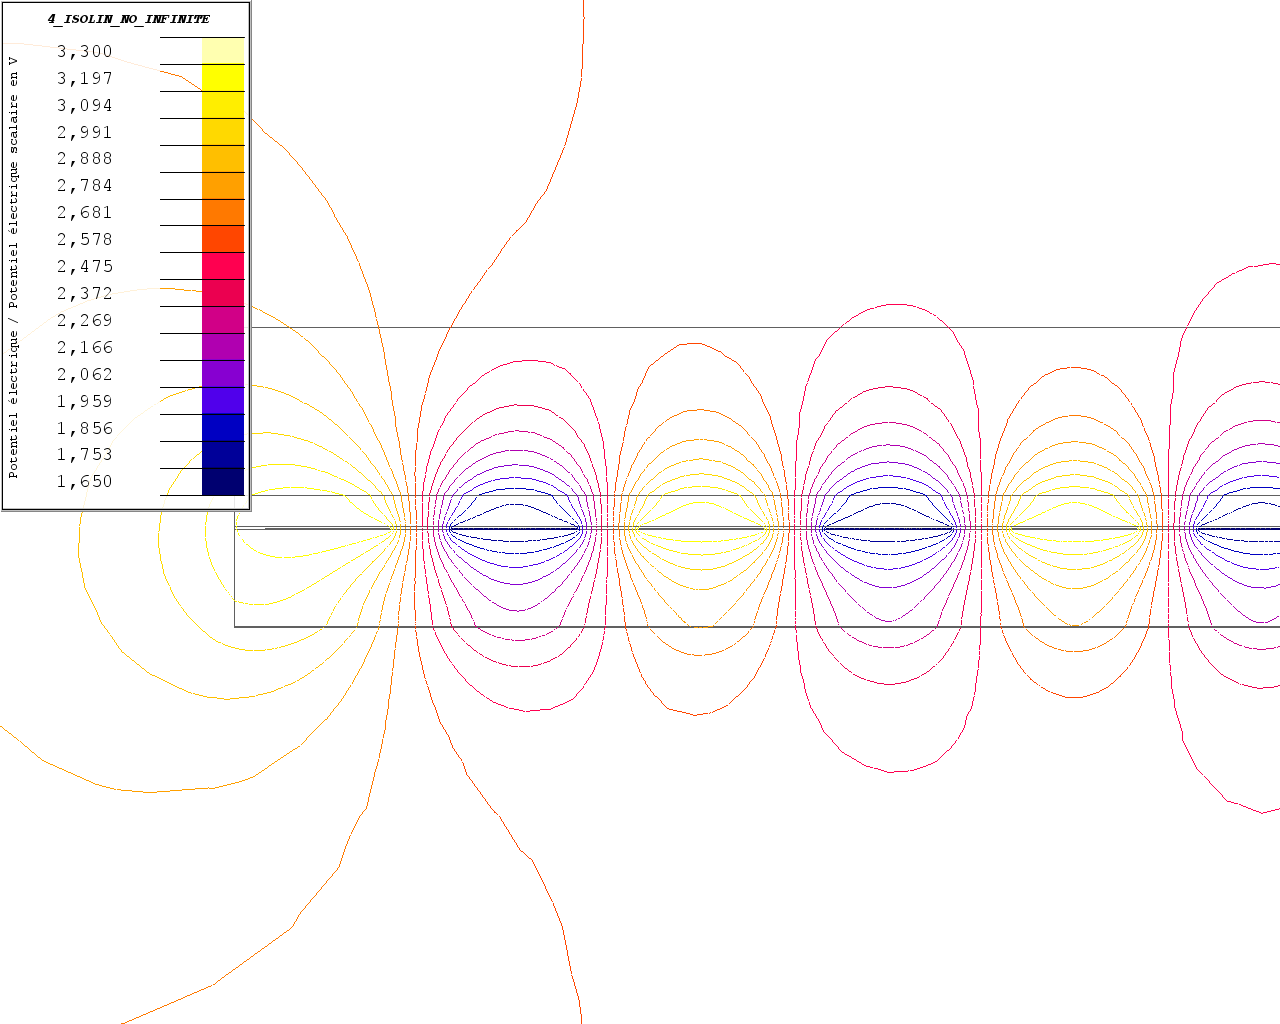
\includegraphics[width=14cm]{C20air.png}
 \caption{Lignes de potentiel électrique 20 pistes}
\end{figure}

On remarque premièrement sur ces graphiques que le maillage est correct. Les lignes sont bien continue même très proche des conducteurs. Les coupure des niveau du champs magnétique sont du à la transition d'un milieux à un autre et sont tout à fait normal. La deuxième information que nous fournis ces figures sont le fait que le champs est bien présent dans l'espace de la cible. Cela veut dire qu'un changement de caractéristique à ce niveau aura une influence sur le champs et donc la capacité. C'est positif pour la viabilité de notre capteur.

Nous pouvons calculé dans cette simulation la capacité de notre système. Nous utilisons pour cela la définition de la capacité qui dépends de l'énergie $C = \frac{2W}{U^2}$. Flux2d intègre tout les point pour calculer l'énergie électrique de tous le modèle en prenant en compte la profondeur spécifié ultérieurement. Nous utilisons notre tension que nous avions mis en paramètre pour attribué notre expressions de la capacité dans un paramètre qu'on appellera C\_total. Ce paramètre sera disponible pour nos prochaine simulation afin d'obtenir directement la valeur et tracer des graphiques. Pour cette première simulation C vaut \SI{78.98}{\pico\farad}. Nous somme au dessus de l'offset maximal de notre convertisseur qui est de 10pF. Nous somme cependant dans le bonne ordre de grandeurs et il ne sera pas dure de diminuer la capacité. 

Nous pouvons jouer avec le rapport distance et largeur de piste afin d'observer comment la capacité varie. Nous créons pour cela un scénario de simulation pour faire varier notre paramètre de 0.5 à 2 sur 10 pas. On remarque bien une diminution de la capacité mais ce n'est pas suffisant. Nous observeront comment elle diminue encore en réduisant le nombre de piste.

\newpage

\begin{figure}[!ht]
 \centering
 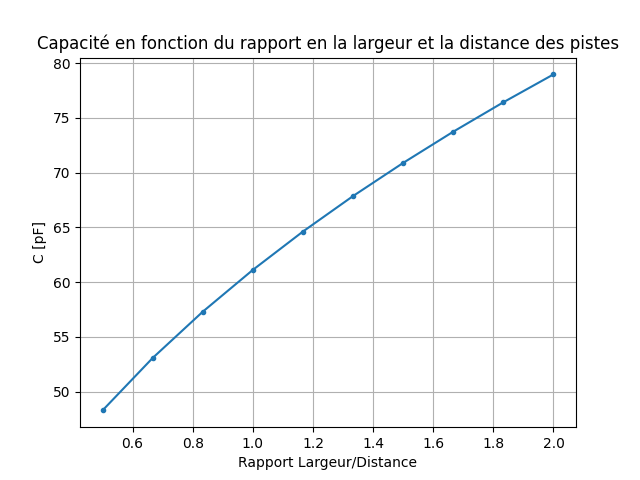
\includegraphics[width=10cm]{C20airGraph.png}
 \caption{Capacité en fonction du rapport distance/largeur}
\end{figure}

Nous allons à présent changer la cible en eau afin d'observer si nous arrivons à la mesurer.


\begin{figure}[!ht]
 \centering
 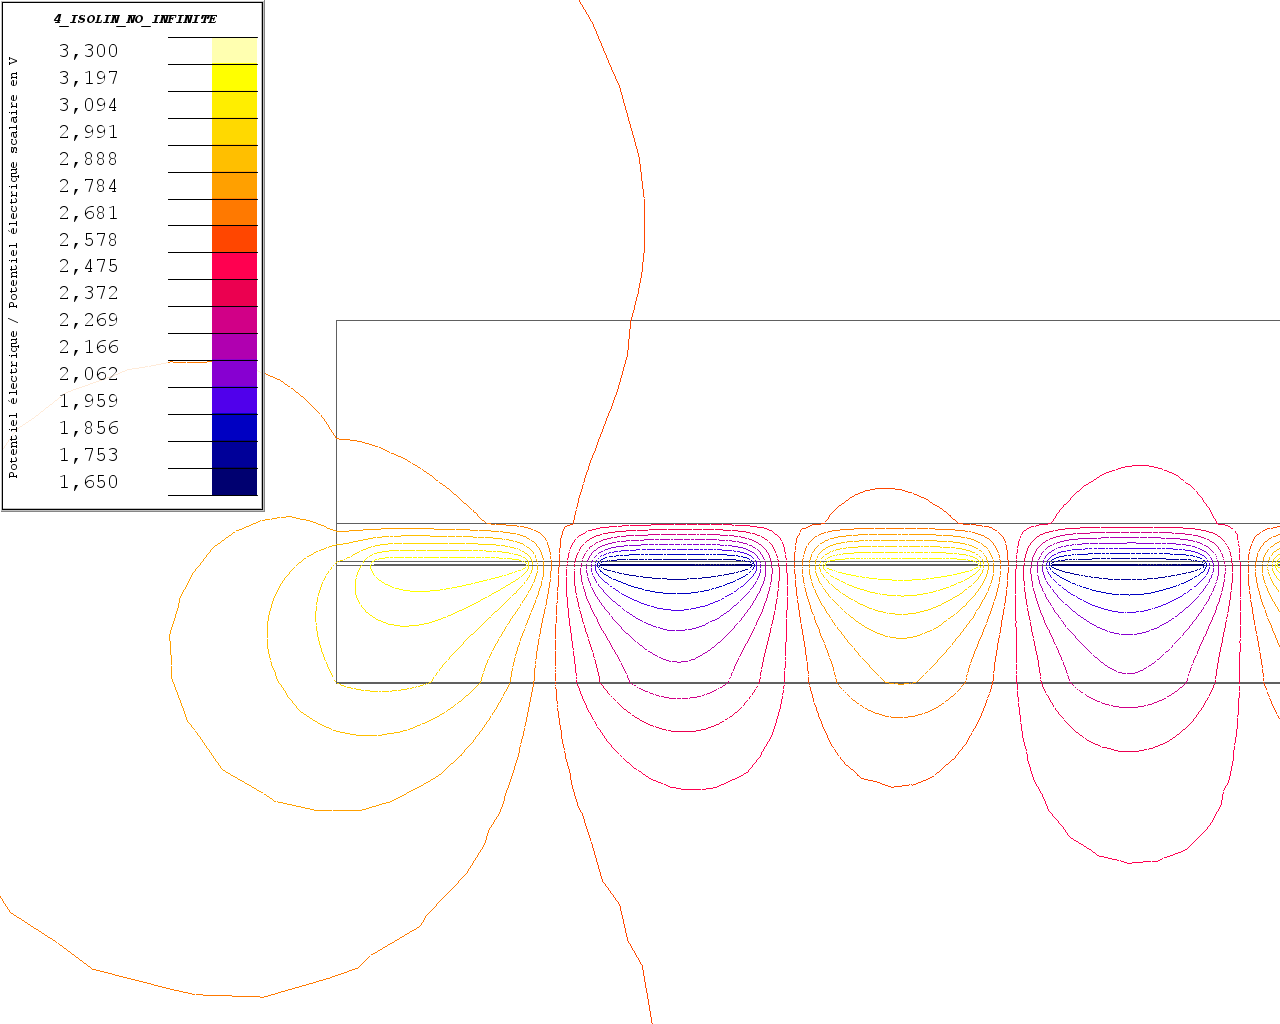
\includegraphics[width=14cm]{C20eauligne.png}
 \caption{Lignes de potentiel électrique 20 pistes avec eau}
 \label{c20eaul}
\end{figure}

\begin{figure}[!ht]
 \centering
 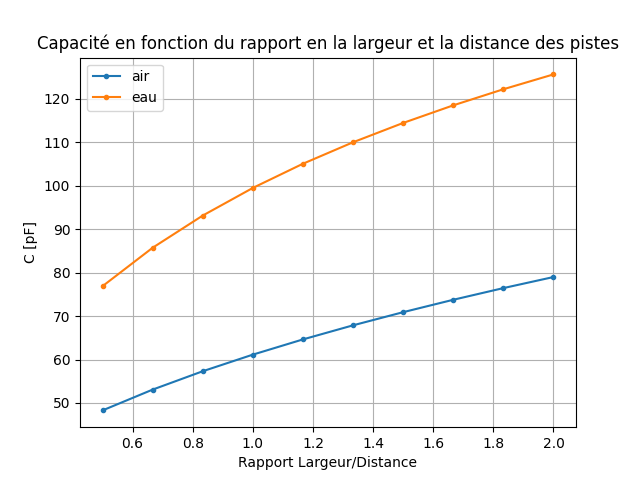
\includegraphics[width=7cm]{C20eauGraph1.png}
 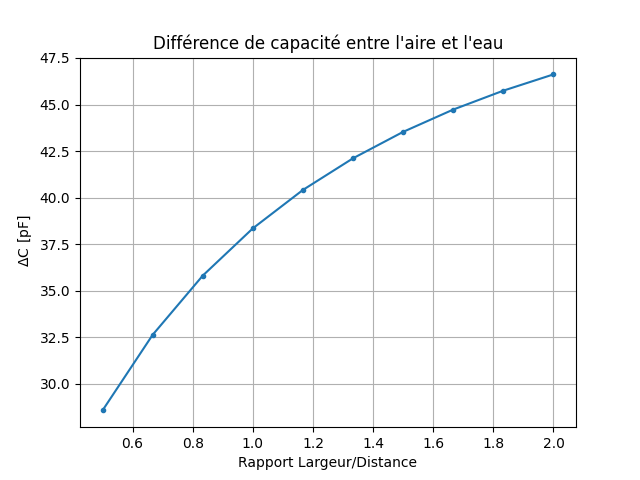
\includegraphics[width=7cm]{C20eauGraph2.png}
 \caption{Comparaison des capacité avec et sans eau pour 20 pistes}
\end{figure}

L'eau modifie bien le champs électrique. On vois sur la figure \ref{c20eaul} que le champs est comprimé. L'effet de l'eau sur la capacité est tout aussi visible. La capacité augmente de près d'un demi de sa valeur. Un fait intéressent est que la différence évolue plus vite que l'offset de capacité. Cela veut dire que si on diminue trop le rapport pour faire diminuer la capacité d'offset on risque de réduire beaucoup trop la sensibilité, bien que nous somme toujours au dessus du seuil de notre convertisseur.

\subsubsection{5 et 10 pistes}
Nous effectuons une simulation avec 5 et 10 piste sur la carte. Nous utilisons toujours le même scénario avec et sans eau.


\begin{figure}[!ht]
 \centering
 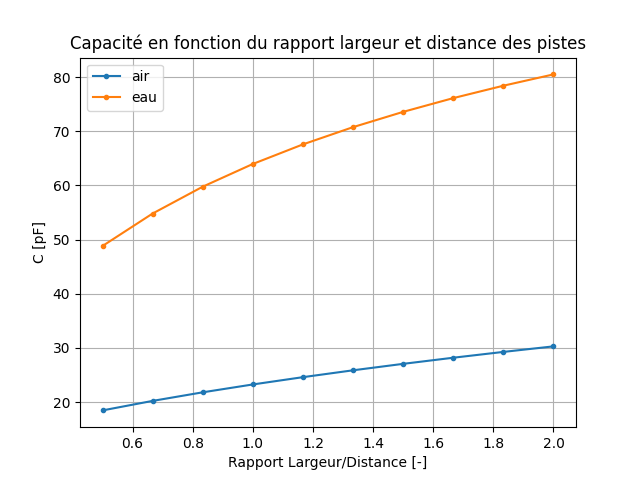
\includegraphics[width=7cm]{C10Graph1.png}
 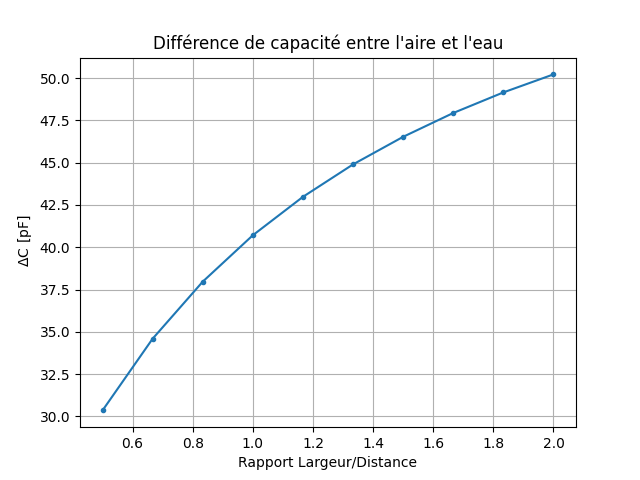
\includegraphics[width=7cm]{C10Graph2.png}
 \caption{Comparaison des capacité avec et sans eau pour 10 pistes}
\end{figure}

Cette nouvelle configuration est meilleur que la première. la capacité d'offset à été divisé par deux tout en gardant un bon delta. Nous somme à présent plus proche des caractéristique du convertisseur.

\begin{figure}[!ht]
 \centering
 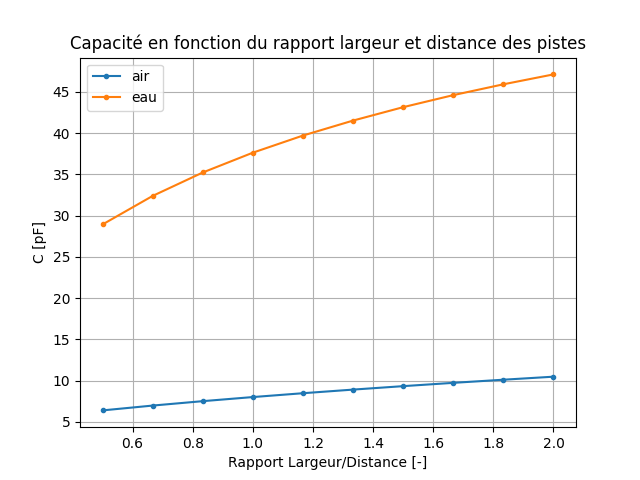
\includegraphics[width=7cm]{C5Graph1.png}
 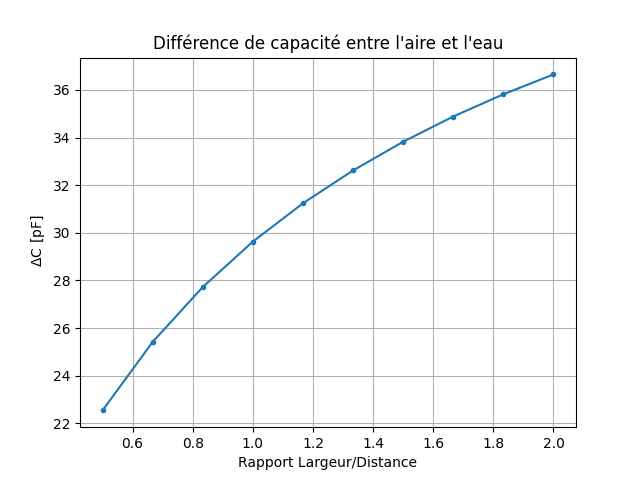
\includegraphics[width=7cm]{C5Graph2.png}
 \caption{Comparaison des capacité avec et sans eau pour 5 pistes}
\end{figure}
\newpage

Grâce à 5 piste nous atteignons enfin la capacité d'offset cherché. La différence de capacité à diminué mais est toujours très élever si on la compare à l'offset. Ces résultat sont a bien considéré car le modèle ne nous permet pas de simulé de fine goutte entre les lignes. Il est donc difficile de prévoir si une carte avec moins de ligne peut capter toutes les goutte. Seul les mesures permettrons de nous le dire. 

\subsubsection{Plan de cuivre}

L'utilisation d'un plan de cuivre à été pensé pour concentrer la mesure à la surface haute de la carte. Nous appliqueront donc un conducteur parfait à la couche sous le pcb. Nous allons simulé l'effet d'un plan seulement sur le modèle à 5 ligne. Ce sera suffisant pour comprendre sont effet. Nous lancerons le même scénario avec et sans eau pour que nous puissions comparer.

\begin{figure}[!ht]
 \centering
 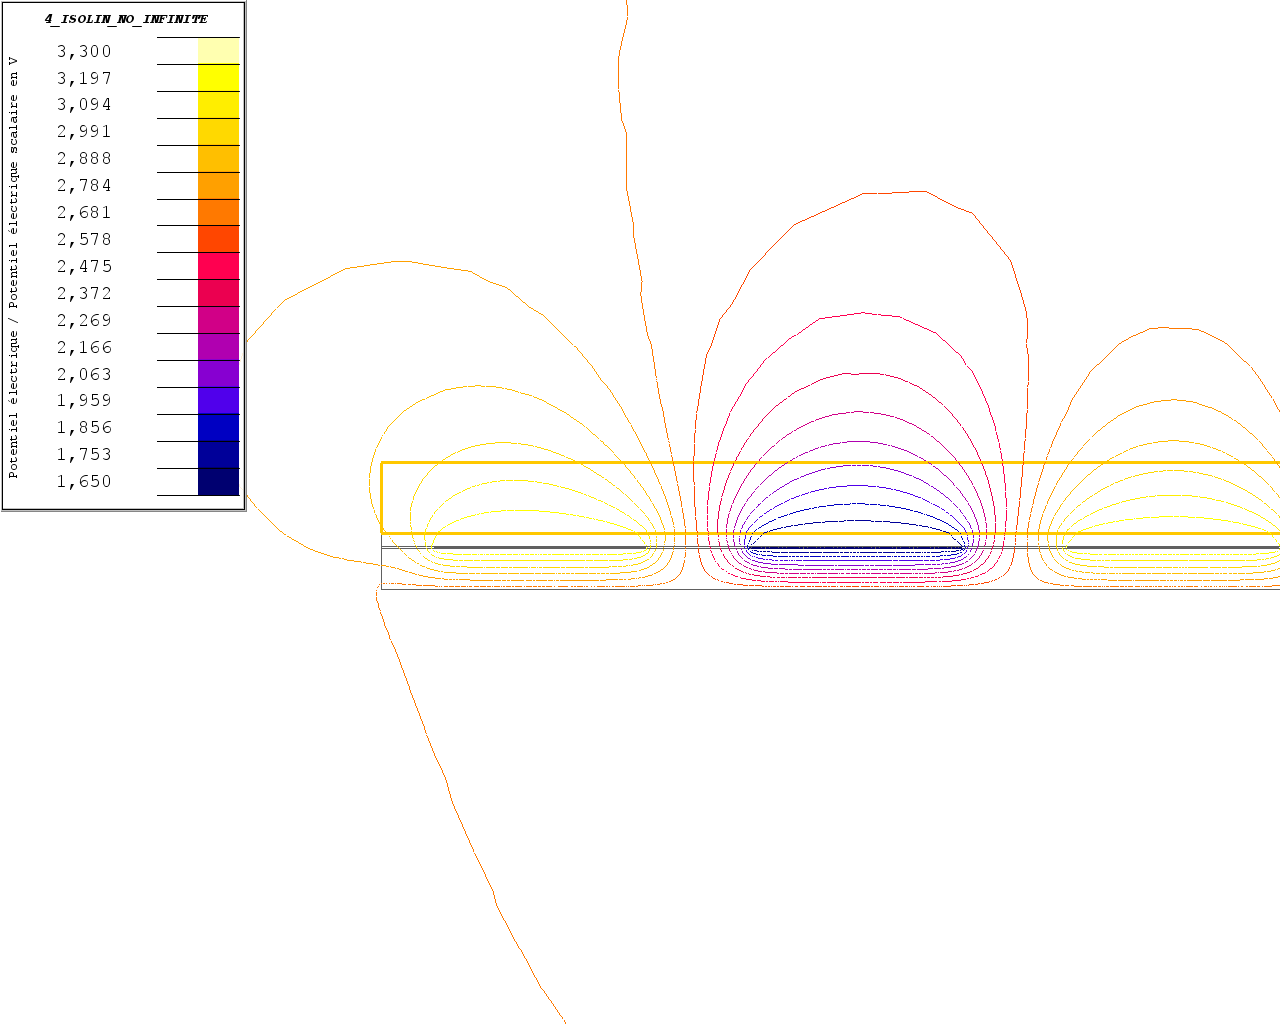
\includegraphics[width=10cm]{C5airMasseligne.png}
 \caption{Lignes de potentiel électrique, avec plan, avec eau pour 5 pistes}
 \label{c5planlair}
\end{figure}

\begin{figure}[!ht]
 \centering
 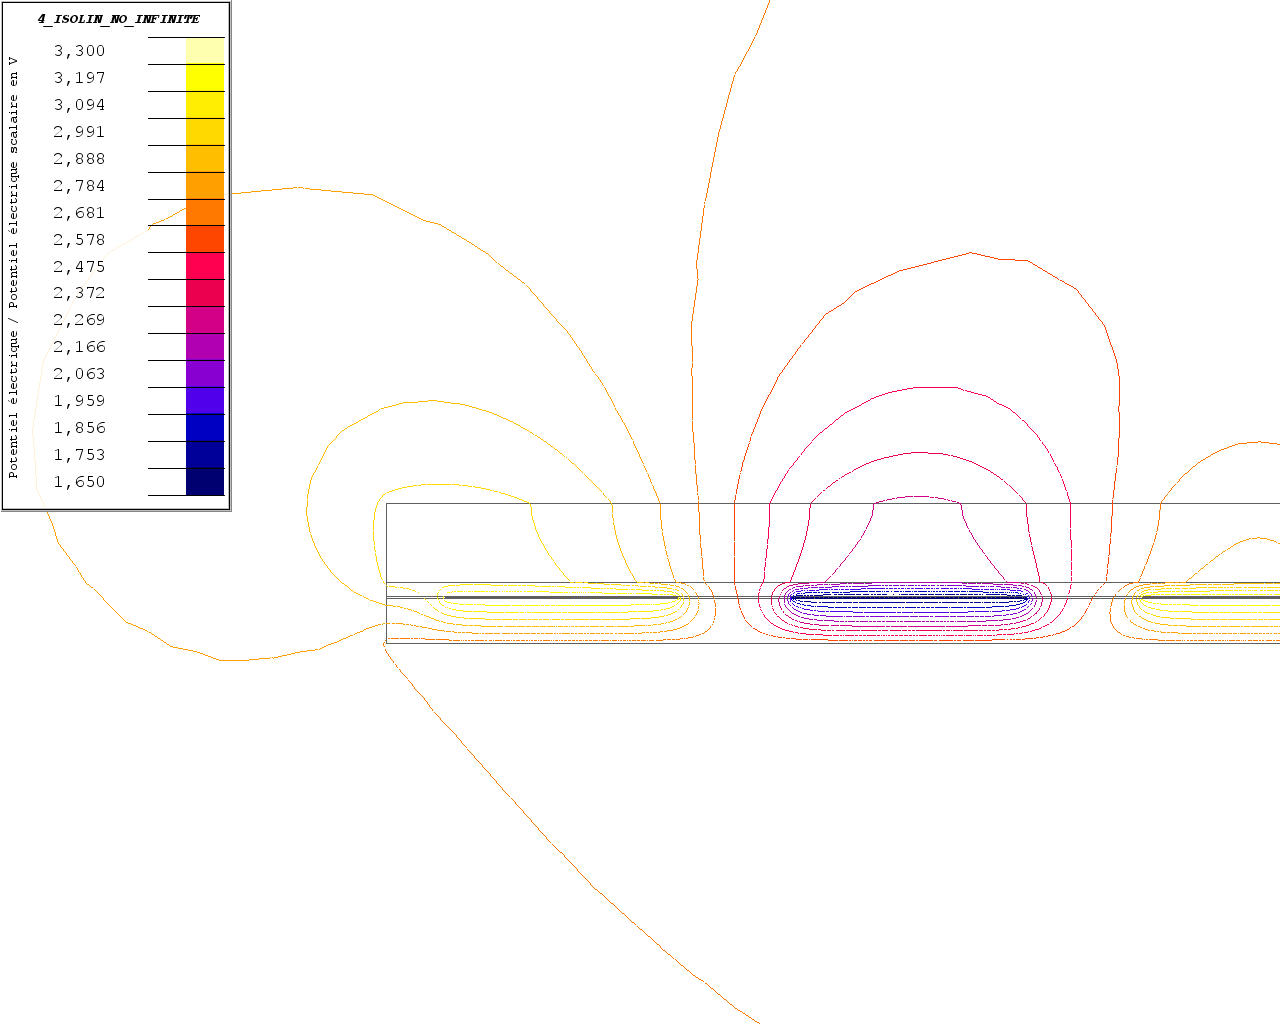
\includegraphics[width=10cm]{C5eauMasseligne.png}
 \caption{Lignes de potentiel électrique, avec plan, sans eau pour 5 pistes}
 \label{c5planleau}
\end{figure}

\newpage

\begin{figure}[!ht]
 \centering
 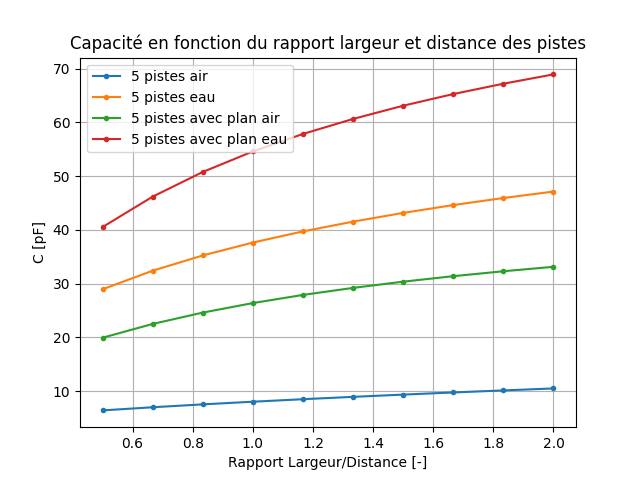
\includegraphics[width=7cm]{C5masseGraph1.png}
 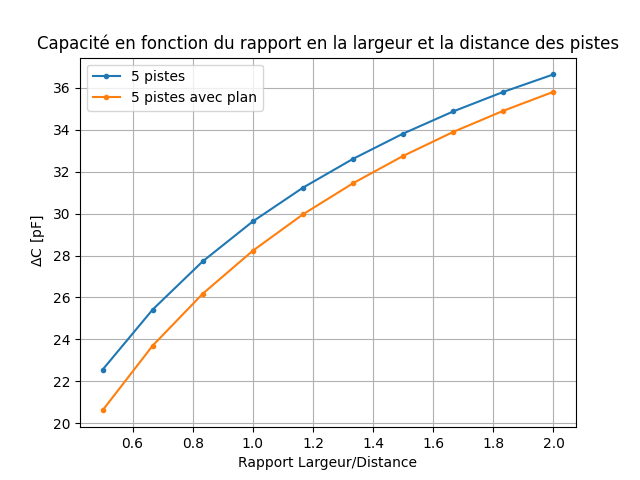
\includegraphics[width=7cm]{C5masseGraph2.png}
 \caption{Comparaison des capacité, avec plan, avec et sans eau pour 5 pistes}
\end{figure}

L'ajout d'un plan augmente l'offset et diminue le delta ce qui n'est pas très intéressant pour nous. Cependant on voit sur la figure \ref{c5planlair} et \ref{c5planleau} que les ligne de potentiel ne sorte plus par dessous. On en déduit que comme prévu tout ce qui se passe en dessous n’influencera plus notre capteur.



\end{document}
